\documentclass{beamer}
%\documentclass[aspectratio=169]{beamer}
%
\mode<presentation>
{
  \usetheme{default}      
  \usecolortheme{default}
  \usefonttheme{default} 
  \setbeamertemplate{navigation symbols}{}
  \setbeamertemplate{caption}[numbered]
} 

\usepackage[english]{babel}
\usepackage[utf8x]{inputenc}
\usepackage{amsmath}
\usepackage{bm}
\usepackage{bbm}

\newcommand{\X}{\mathcal{X}}
\newcommand{\Y}{\mathcal{Y}}
\newcommand{\real}{\mathbb{R}}
\newcommand{\N}{\mathbb{N}}
\newcommand{\yhat}{\hat{y}}
\newcommand{\bxi}{\bm{x}^{(i)}}
\newcommand{\bx}{\bm{x}}
\newcommand{\xij}{x^{(i)}_j}
\newcommand{\yi}{y^{(i)}}
\newcommand{\yhati}{\hat{y}^{(i)}}
\newcommand{\norm}[1]{\left\lVert#1\right\rVert}
\newcommand{\1}[1]{\mathbbm{1}\left[#1\right]}

\title[Course presentation]{Machine learning from scratch}
\subtitle{Lecture 5: Linear regression: Recap}
\author{Alexis Zubiolo\newline\texttt{alexis.zubiolo@gmail.com}}
\institute{Data Science Team Lead @ Adcash}
\date{February 2, 2017}

\begin{document}

\begin{frame}
  \titlepage
\end{frame}

\begin{frame}{Information}
All the code that implement what is in this presentation can be found on the GitHub repository (lecture 4, \texttt{least-squares.ipynb}).
\pause
\vfill
The goal of this lecture is to recap what we have seen and list the lessons to remember.
\end{frame}

\begin{frame}{OLS recap}
\textbf{Data}: features $x \in \X$ (size and intercept), labels $y \in \Y$ (prices)

\textbf{Linear model}: $\hat{y} = h(x) = \theta^T x$

\textbf{Loss function}:
\begin{equation*}
J(\theta) = \dfrac{1}{2} \sum_{i = 1}^{n} \left( h\left(\bxi\right) - \yi \right)^2
\end{equation*}

\textbf{Gradient}: 
\begin{equation*}
\nabla J(\theta) = \left[ \dfrac{\partial}{\partial \theta_1} J(\theta), \dots, \dfrac{\partial}{\partial \theta_d} J(\theta) \right]^T
\end{equation*}
where
\begin{equation*}
\dfrac{\partial}{\partial \theta_j} J(\theta) = \sum_{i = 1}^{d}\left( h\left(\bxi\right) - \yi \right) x^{(i)}_j
\end{equation*}
\textbf{Update rule}:
\begin{equation*}
\theta_j := \theta_j - \alpha \dfrac{\partial}{\partial \theta_j} J(\theta)
\end{equation*}
\end{frame}

\begin{frame}{Batch vs. Stochastic gradient descent}
The update rule:
\begin{equation*}
\theta_j := \theta_j - \alpha \dfrac{\partial}{\partial \theta_j} J(\theta)
\end{equation*}
where
\begin{equation*}
\dfrac{\partial}{\partial \theta_j} J(\theta) = \sum_{i = 1}^{d}\left( h\left(\bxi\right) - \yi \right) x^{(i)}_j
\end{equation*}
is called \textbf{batch update gradient descent} because the gradient is computed on \textbf{the whole training set}. \pause For some $i$, the update rule 
\begin{equation*}
\theta_j := \theta_j - \alpha \dfrac{\partial}{\partial \theta_j} J^{(i)}(\theta)
\end{equation*}
where
\begin{equation*}
\dfrac{\partial}{\partial \theta_j} J^{(i)}(\theta) = \left( h\left(\bxi\right) - \yi \right) x^{(i)}_j
\end{equation*}
is called \textbf{stochastic gradient descent} because the gradient is computed on \textbf{a single sample}.
\end{frame}

\begin{frame}{Rescaling the data} 
In our example:
\begin{itemize}
	\item The intercept is constantly equal to 1
	\item The size of the house varies between $\approx$ 10 and $\approx$ 100
\end{itemize}
Hence, there is a 10-100 difference in order of magnitude between the 2 variables, and the loss function looks like: 
\begin{figure}
\centering
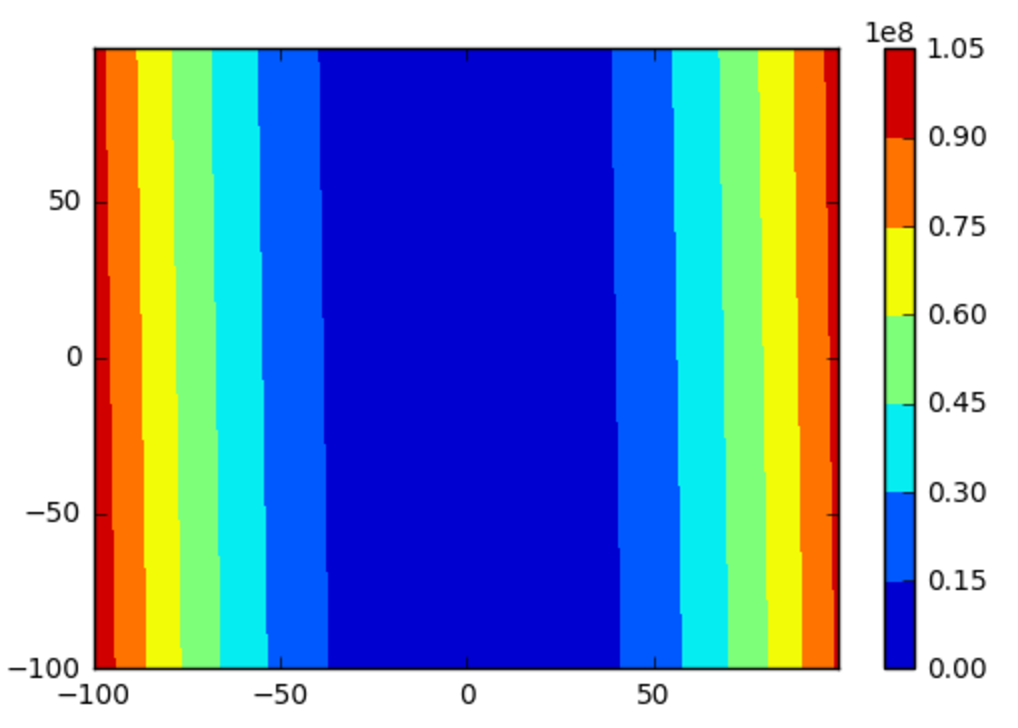
\includegraphics[width=.6\linewidth]{images/unnormalized_loss.png}
\end{figure}
which means the function varies much faster over an axis ($\theta_1 = $ price) than the other ($\theta_0 = $ intercept).
\end{frame}

\begin{frame}{Rescaling the data}
To avoid this issue, rescaling (or standardizing) the data can help. One way to do it is:
$$ z = \dfrac{x - x_{\min}}{x_{\max} - x_{\min}} $$
and replace $x$ by $z$ in $J$. Hence, we get a loss function that looks like that:
\begin{figure}
\centering
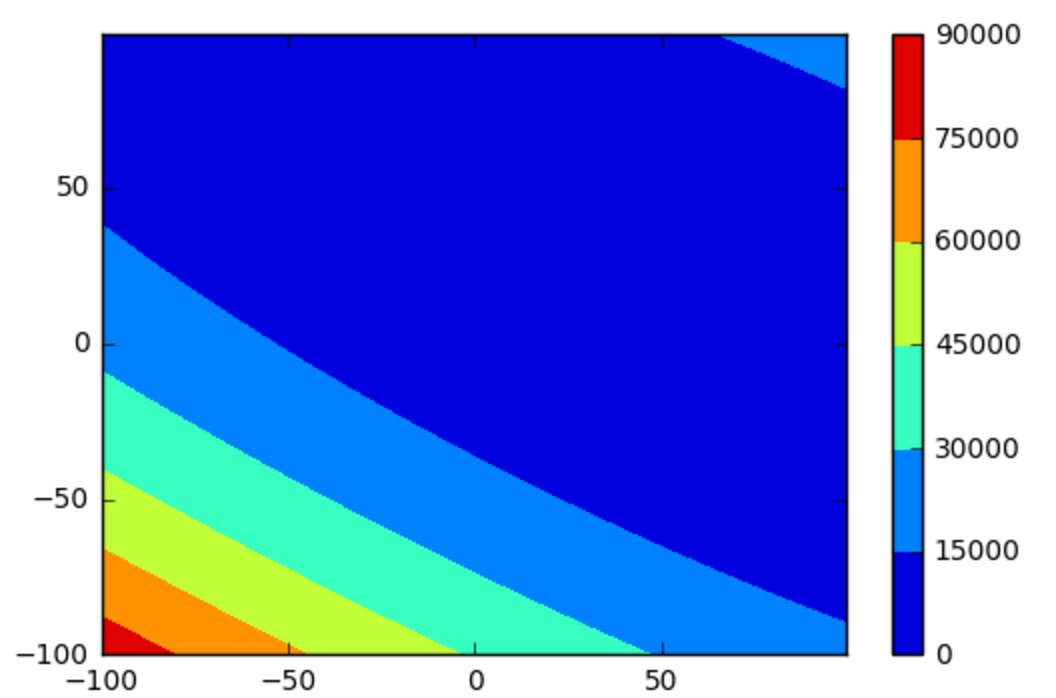
\includegraphics[width=.6\linewidth]{images/normalized_loss.png}
\end{figure}
Here, both variable have roughly the same importance. In general, it makes the optimization step much more stable and faster.
\end{frame}

\begin{frame}{Learning rate choice}
We also saw that the choice of the learning rate was \textbf{crucial}. It can be:
\begin{itemize}
	\item \textbf{Too big} and the optimization can \textbf{diverge}
	\item \textbf{Too small} and the optimization can be \textbf{slow}
	\item Properly tuned to have a \textbf{fast convergence}
\end{itemize}
\begin{figure}
\centering
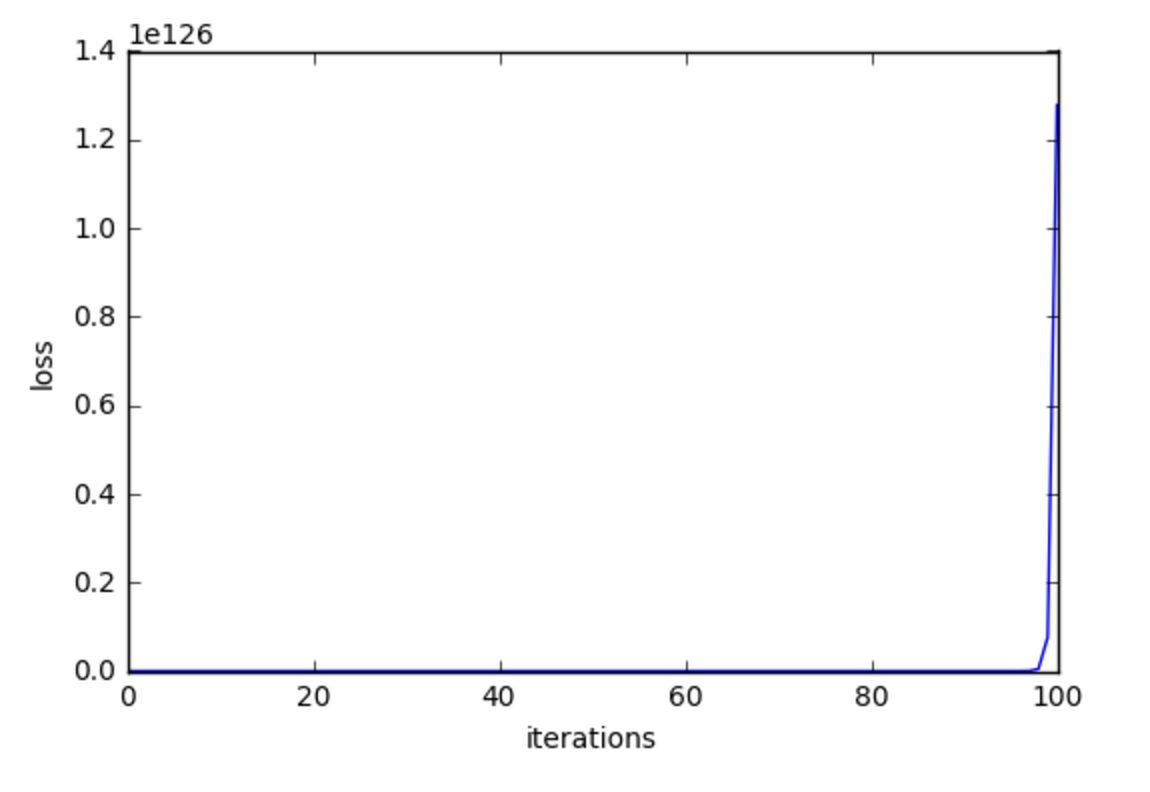
\includegraphics[width=.3\linewidth]{images/alpha_big.png}~
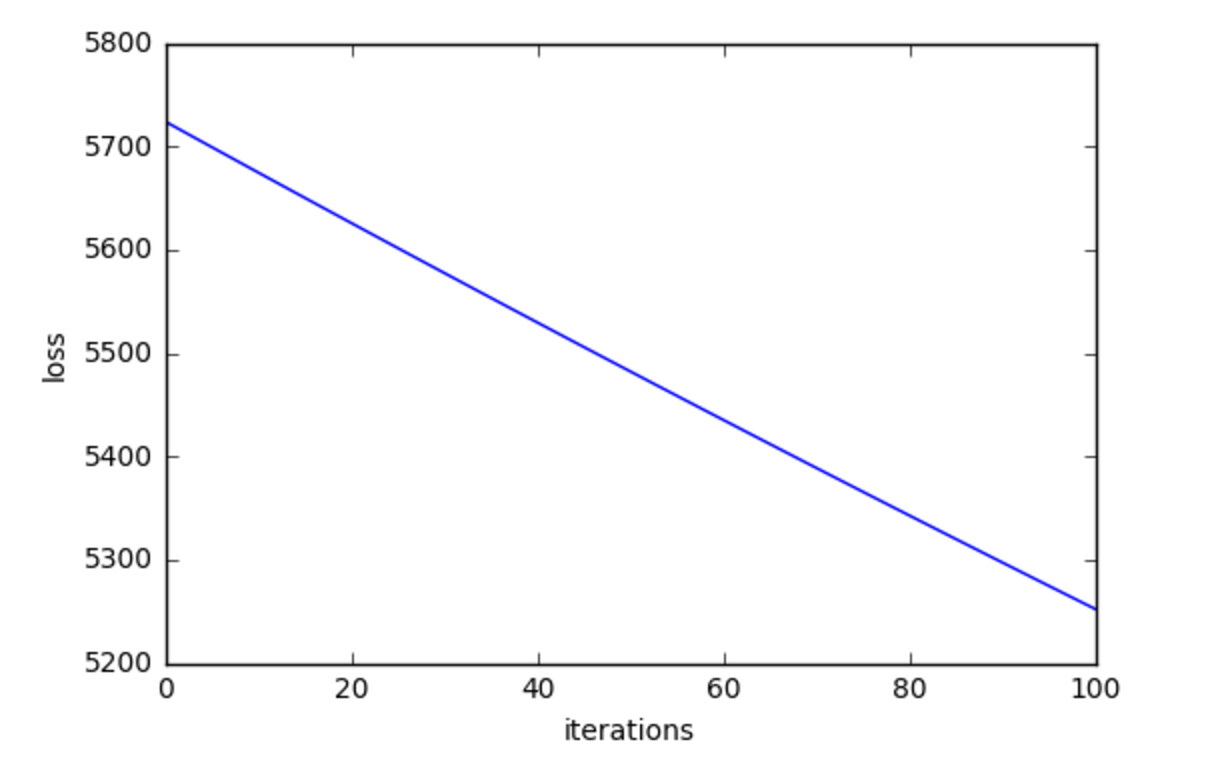
\includegraphics[width=.3\linewidth]{images/alpha_small.png}~
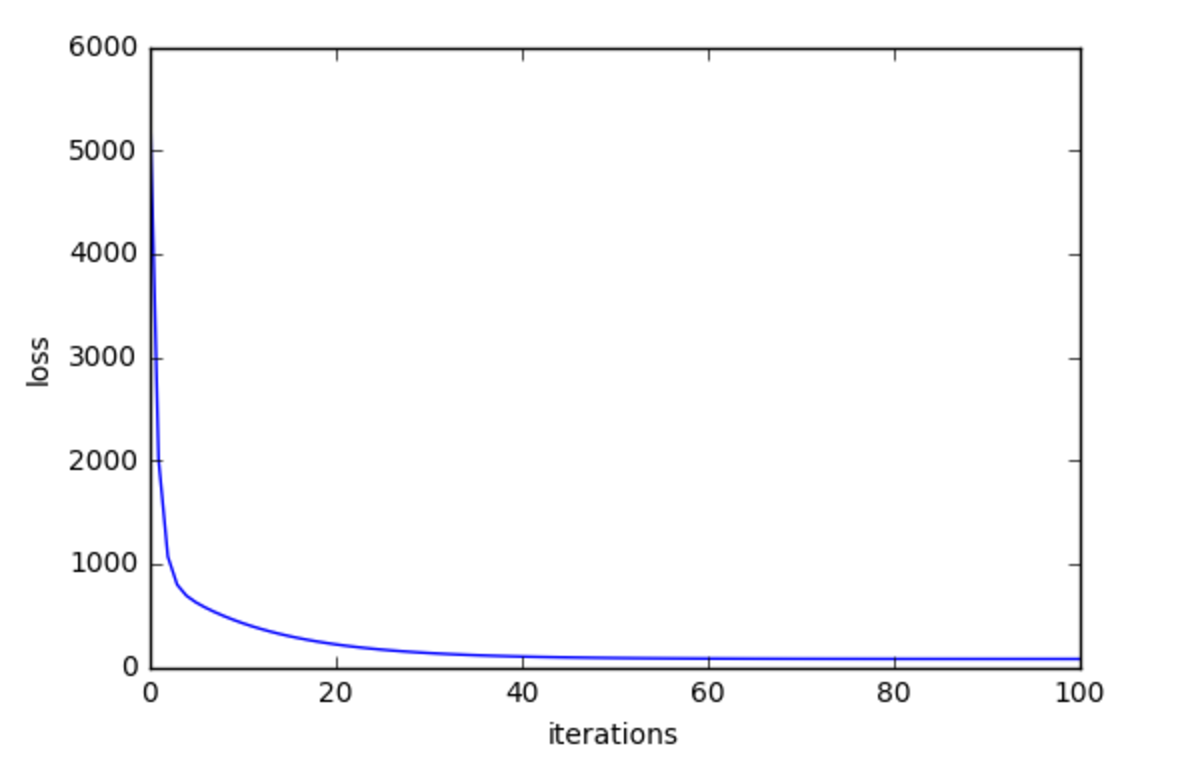
\includegraphics[width=.3\linewidth]{images/alpha_ok.png}
\end{figure}
\end{frame}

\begin{frame}{Decreasing learning rate}
In stochastic gradient descent, we sometimes saw the loss function \textbf{going up and down in the end}: 
\begin{figure}
\centering
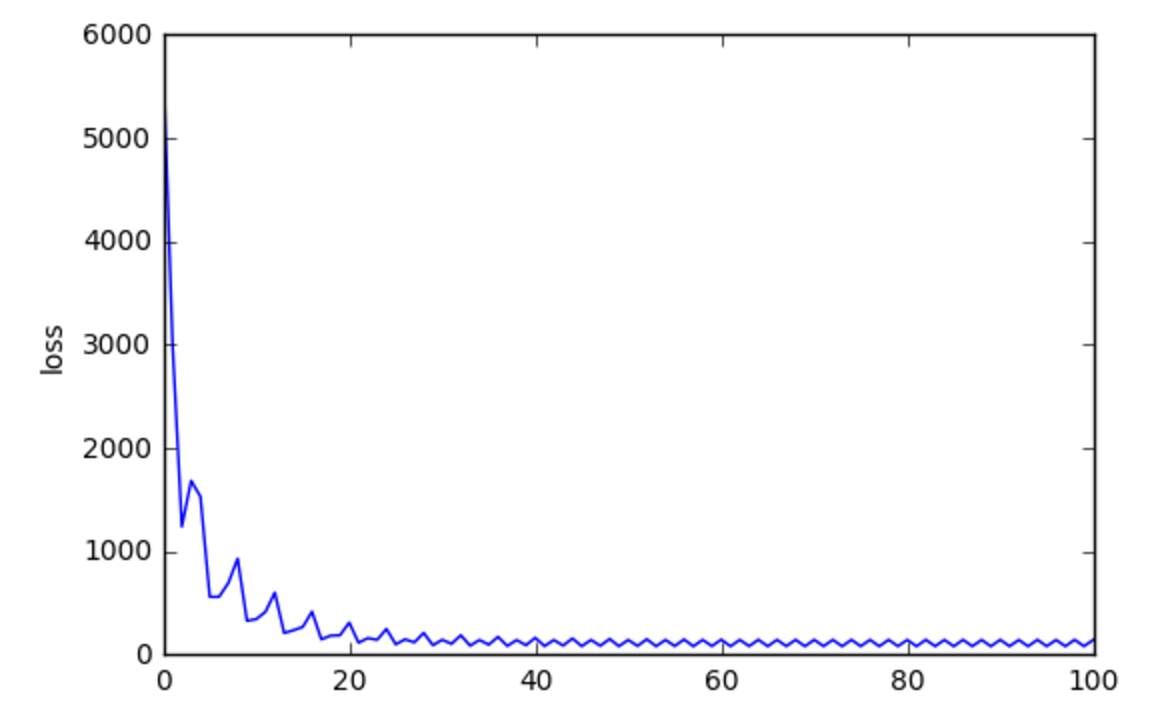
\includegraphics[width=.8\linewidth]{images/sgd_constant_alpha.png}
\end{figure}
This is because the $d$ loss functions $J^{(i)}(\theta)$ for $i = 1, 2, 3 \text{~or~} 4$ have different optimal $\theta$.
\end{frame}

\begin{frame}{Decreasing learning rate}
One way to avoid it is to set a \textbf{decreasing learning rate} that would go to 0 when the number of the current iteration $i$ goes to infinity. Example$$\alpha_i = \dfrac{1}{i+1} \quad \text{or} \quad \alpha_i = \dfrac{1}{\sqrt{i+1}}$$
\begin{figure}
\centering
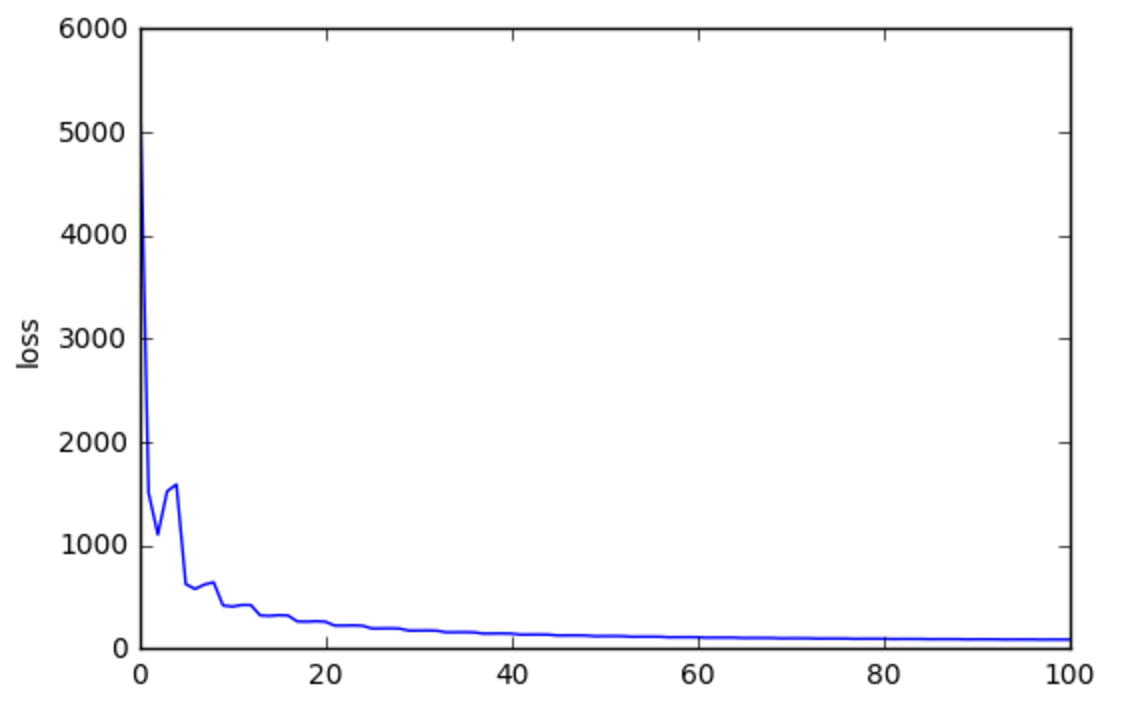
\includegraphics[width=.8\linewidth]{images/sgd_decreasing_alpha.png}
\end{figure}
\end{frame}

\begin{frame}{Another way to track the evolution of the optimization}
We can plot the loss function (in 2D) and show where $\theta$ is at each iteration. Example with the standard gradient descent:
\begin{figure}
\centering
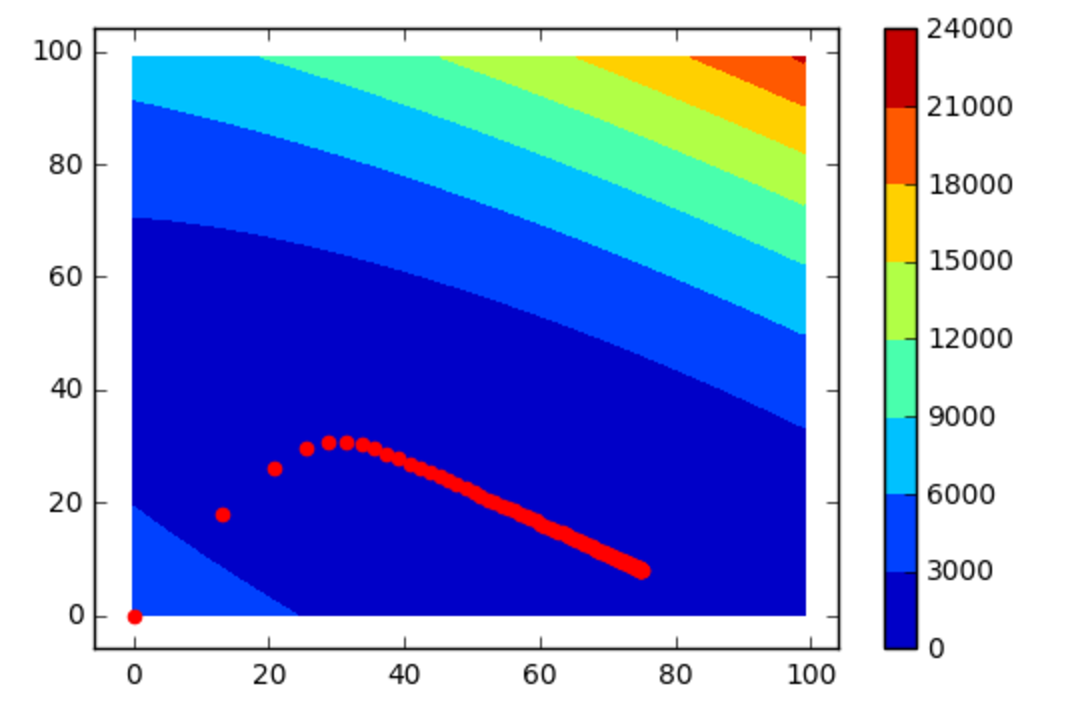
\includegraphics[width=\linewidth]{images/theta_evolution_gd.png}
\end{figure}
\end{frame}

\begin{frame}{Another way to track the evolution of the optimization}
Example with the stochastic gradient descent with constant learning rate:
\begin{figure}
\centering
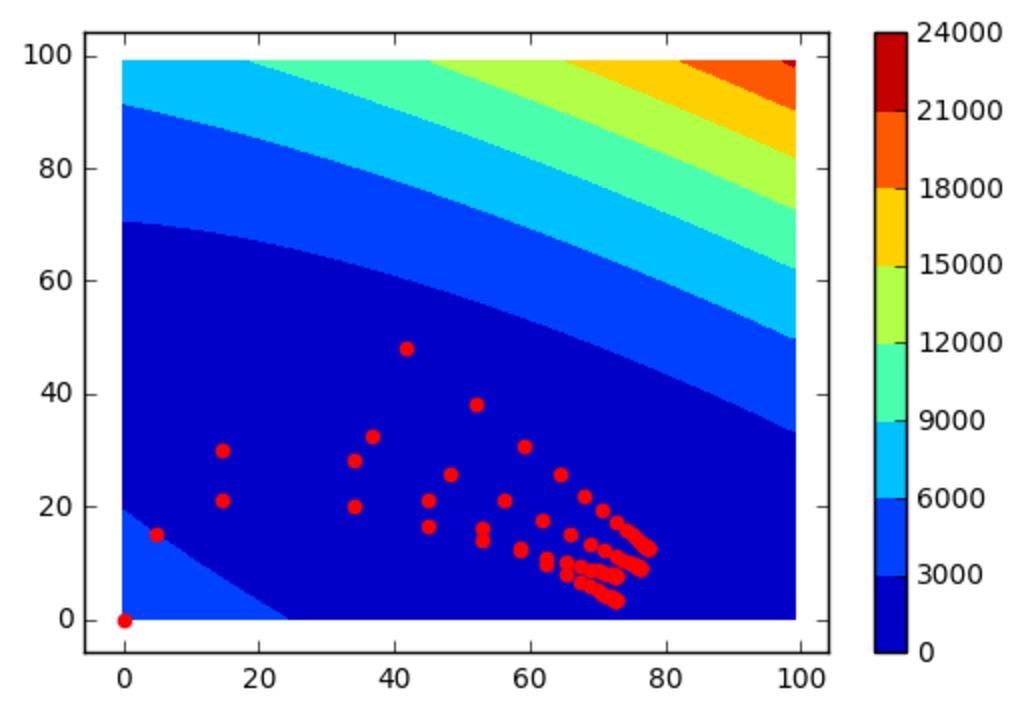
\includegraphics[width=\linewidth]{images/theta_evolution_sgd_constant_alpha.png}
\end{figure}
\end{frame}

\begin{frame}{Another way to track the evolution of the optimization}
Example with the stochastic gradient descent with decreasing learning rate:
\begin{figure}
\centering
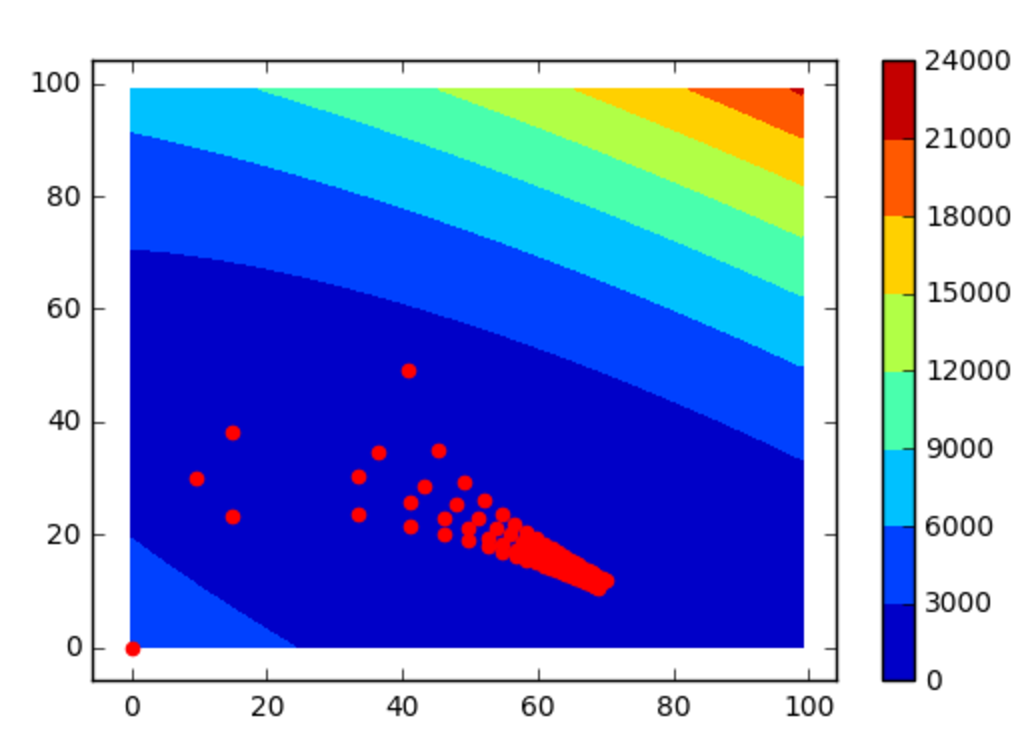
\includegraphics[width=\linewidth]{images/theta_evolution_sgd_decreasing_alpha.png}
\end{figure}
\end{frame}

\begin{frame}{Outliers, overfitting and regularization}
If we look at the regression model we've trained, it looks like that \ldots
\begin{figure}
\centering
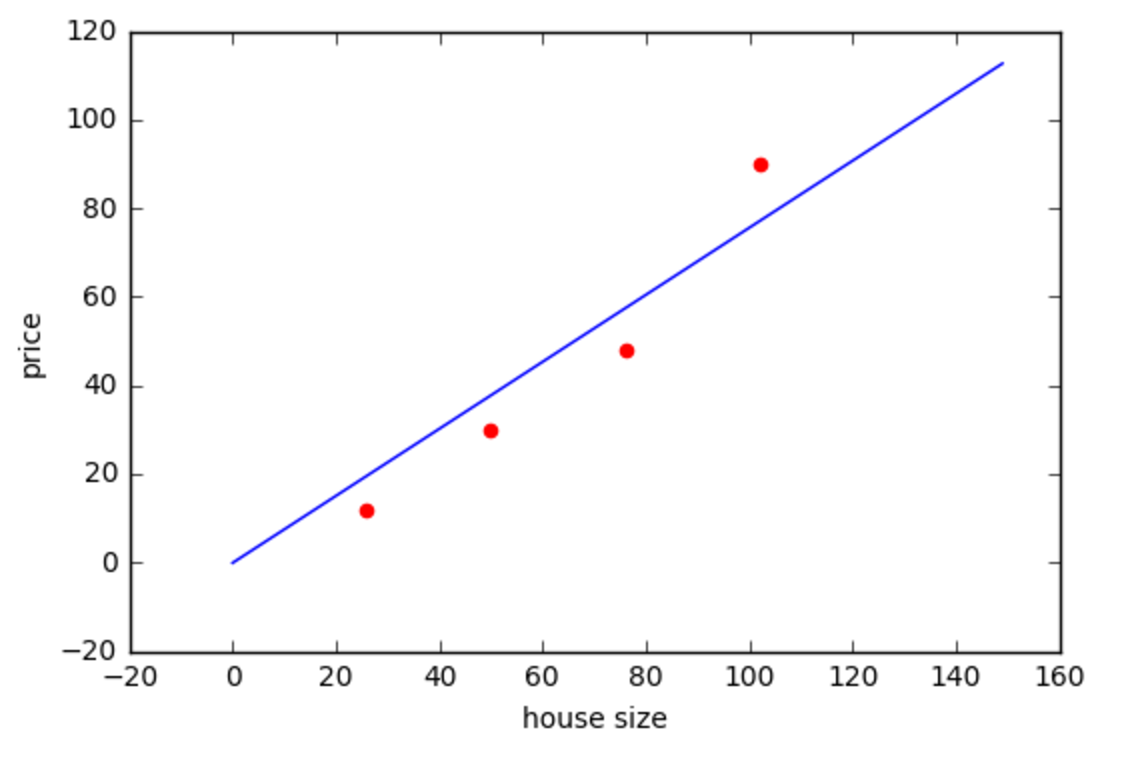
\includegraphics[width=\linewidth]{images/line_regression.png}
\end{figure}
\end{frame}

\begin{frame}{Outliers, overfitting and regularization}
\ldots{} but if we change the price of the latest house to, say, 300k instead of 90k (in this case it becomes an \textbf{outlier}), we would have:
\begin{figure}
\centering
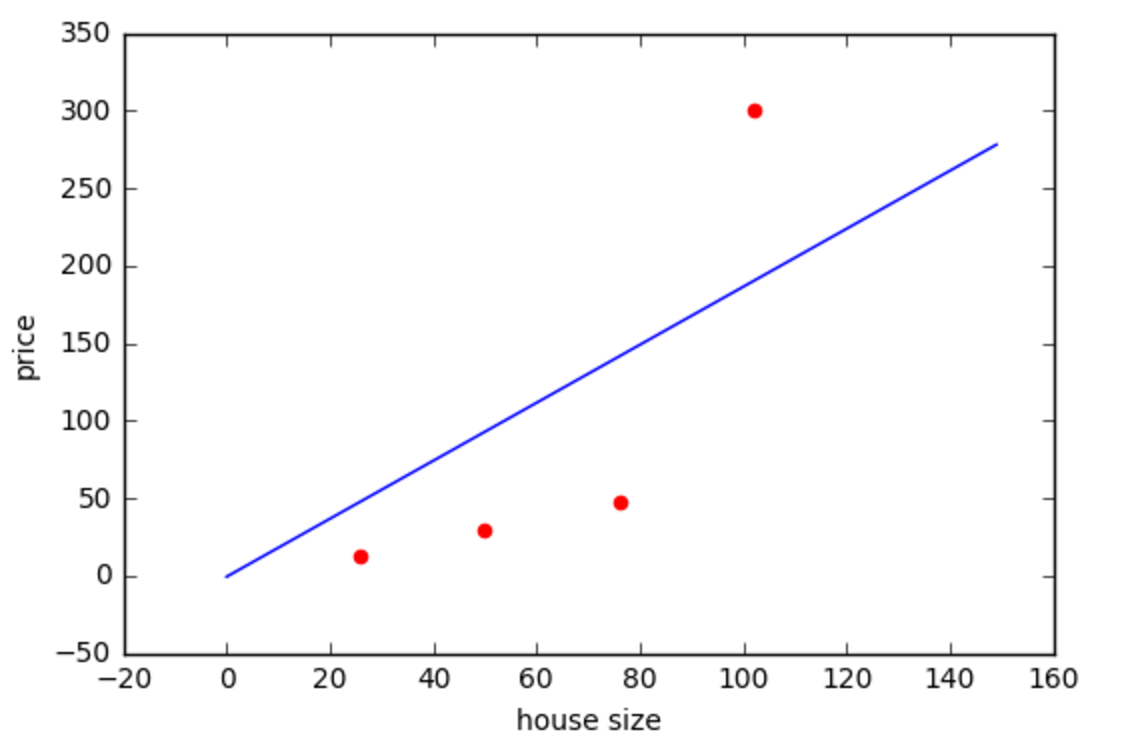
\includegraphics[width=\linewidth]{images/line_regression_outlier.png}
\end{figure}
\end{frame}

\begin{frame}{Outliers, overfitting and regularization}
This means we are trying too hard to fit the outlier. 
\pause
\vfill
This phenomenon is called \textbf{overfitting}. In this case, we generally notice some of the coefficients are very big. Hence, a way to avoid overfitting is to penalize too big coefficients. This can be 

\end{frame}

\begin{frame}{Conclusion and next session}
We've reviewed the main steps of the ordinary least-squares. The steps are often the same:
\begin{itemize}
	\item Define a model (linear in OLS)
	\item Define a loss function
	\item Optimize the loss function
\end{itemize}
\pause
\vfill
What's next?
\begin{itemize}
	\item Implementation of regularization
	\item Implementation of more sophisticated models
	\item Extension to classification
\end{itemize}
\end{frame}

\begin{frame}
\vfill
\centering
\begin{huge}
\huge{Thank you! Questions?}
\vfill
\texttt{alexis.zubiolo@gmail.com}
\end{huge}
\vfill
\begin{Large}
\texttt{https://github.com/azubiolo/itstep}
\end{Large}
\vfill
\end{frame}

\end{document}
